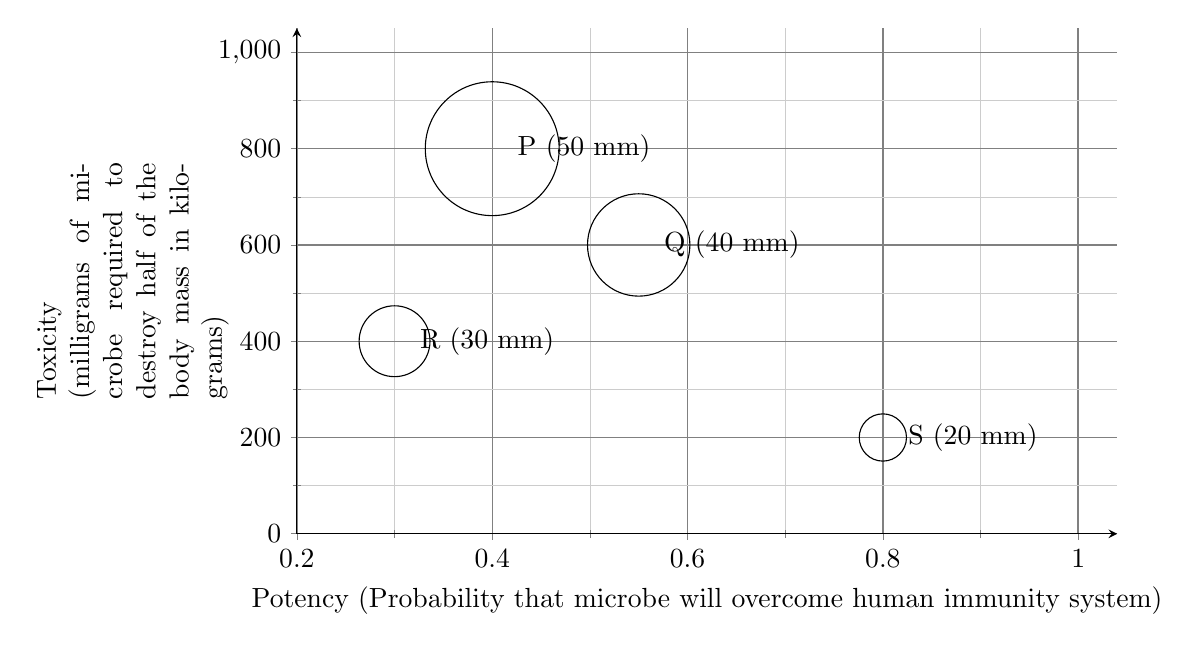
\begin{tikzpicture}
\begin{axis}[
    width=12cm,
    height=8cm,
    xlabel={Potency (Probability that microbe will overcome human immunity system)},
    ylabel style={at={(axis description cs:-0.2,0.5)}, anchor=center},
    ylabel={\parbox{3cm}{Toxicity \\ (milligrams of microbe required to destroy half of the body mass in kilograms)}},
    ymin=0, ymax=1000,
    xmin=0.2, xmax=1,
    ytick={0,200,400,600,800,1000},
    xtick={0.2,0.4,0.6,0.8,1},
    grid=both,
    minor tick num=1,
    major grid style={line width=0.5pt,draw=black!50},
    minor grid style={line width=0.2pt,draw=black!20},
    axis lines=left,
    enlarge y limits={value=0.05,upper},
    enlarge x limits={value=0.05,upper},
]

% Circles with labels and values beside them, positioned according to the image
\draw[black] (axis cs:0.4,800) circle (0.85cm);
\node[anchor=west, xshift=0.2cm] at (axis cs:0.4,800) {P (50 mm)};

\draw[black] (axis cs:0.55,600) circle (0.65cm);
\node[anchor=west, xshift=0.2cm] at (axis cs:0.55,600) {Q (40 mm)};

\draw[black] (axis cs:0.3,400) circle (0.45cm);
\node[anchor=west, xshift=0.2cm] at (axis cs:0.3,400) {R (30 mm)};

\draw[black] (axis cs:0.8,200) circle (0.3cm);
\node[anchor=west, xshift=0.2cm] at (axis cs:0.8,200) {S (20 mm)};

\end{axis}
\end{tikzpicture}
